\documentclass[t]{beamer}

\subtitle{Section 1.2: Divisors and Prime Factorization}

\usepackage{amsthm,amsmath,amsfonts,hyperref,graphicx,color,multicol,soul}
\usepackage{enumitem,tikz,tikz-cd,setspace,mathtools}

%%%%%%%%%%
%Beamer Template Customization
%%%%%%%%%%
\setbeamertemplate{navigation symbols}{}
\setbeamertemplate{theorems}[ams style]
\setbeamertemplate{blocks}[rounded]

\definecolor{Blu}{RGB}{43,62,133} % UWEC Blue
\setbeamercolor{structure}{fg=Blu} % Titles

%Unnumbered footnotes:
\newcommand{\blfootnote}[1]{%
	\begingroup
	\renewcommand\thefootnote{}\footnote{#1}%
	\addtocounter{footnote}{-1}%
	\endgroup
}

%%%%%%%%%%
%TikZ Stuff
%%%%%%%%%%
\usetikzlibrary{arrows}
\usetikzlibrary{shapes.geometric}
\tikzset{
	smaller/.style={
		draw,
		regular polygon,
		regular polygon sides=3,
		fill=white,
		node distance=2cm,
		minimum height=1in,
		line width = 2pt
	}
}
\tikzset{
	smsquare/.style={
		draw,
		regular polygon,
		regular polygon sides=4,
		fill=white,
		node distance=2cm,
		minimum height=1in,
		line width = 2pt
	}
}


%%%%%%%%%%
%Custom Commands
%%%%%%%%%%

\newcommand{\C}{\mathbb{C}}
\newcommand{\quats}{\mathbb{H}}
\newcommand{\N}{\mathbb{N}}
\newcommand{\Q}{\mathbb{Q}}
\newcommand{\R}{\mathbb{R}}
\newcommand{\Z}{\mathbb{Z}}

\newcommand{\ds}{\displaystyle}

\newcommand{\fn}{\insertframenumber}

\newcommand{\id}{\operatorname{id}}
\newcommand{\im}{\operatorname{im}}
\newcommand{\Aut}{\operatorname{Aut}}
\newcommand{\Inn}{\operatorname{Inn}}

\newcommand{\blank}[1]{\underline{\hspace*{#1}}}

\newcommand{\abar}{\overline{a}}
\newcommand{\bbar}{\overline{b}}
\newcommand{\cbar}{\overline{c}}

\newcommand{\nml}{\unlhd}

%%%%%%%%%%
%Custom Theorem Environments
%%%%%%%%%%
\theoremstyle{definition}
\newtheorem{exercise}{Exercise}
\newtheorem{question}[exercise]{Question}
\newtheorem{warmup}{Warm-Up}
\newtheorem*{defn}{Definition}
\newtheorem*{exa}{Example}
\newtheorem*{disc}{Group Discussion}
\newtheorem*{nb}{Note}
\newtheorem*{recall}{Recall}
\renewcommand{\emph}[1]{{\color{blue}\texttt{#1}}}

\definecolor{Gold}{RGB}{237, 172, 26}
%Statement block
\newenvironment{statementblock}[1]{%
	\setbeamercolor{block body}{bg=Gold!20}
	\setbeamercolor{block title}{bg=Gold}
	\begin{block}{\textbf{#1.}}}{\end{block}}
\newenvironment{thm}[1]{%
	\setbeamercolor{block body}{bg=Gold!20}
	\setbeamercolor{block title}{bg=Gold}
	\begin{block}{\textbf{Theorem #1.}}}{\end{block}}


%%%%%%%%%%
%Custom Environment Wrappers
%%%%%%%%%%
\newcommand{\enumarabic}[1]{
	\begin{enumerate}[label=\textbf{\arabic*.}]
		#1
	\end{enumerate}
}
\newcommand{\enumalph}[1]{
	\begin{enumerate}[label=(\alph*)]
		#1
	\end{enumerate}
}
\newcommand{\bulletize}[1]{
	\begin{itemize}[label=$\bullet$]
		#1
	\end{itemize}
}
\newcommand{\circtize}[1]{
	\begin{itemize}[label=$\circ$]
		#1
	\end{itemize}
}
\newcommand{\slide}[1]{
	\begin{frame}{\fn}
		#1
	\end{frame}
}
\newcommand{\slidec}[1]{
\begin{frame}[c]{\fn}
	#1
\end{frame}
}
\newcommand{\slidet}[2]{
	\begin{frame}{\fn\ - #1}
		#2
	\end{frame}
}


\newcommand{\startdoc}{
		\title{Math 425: Abstract Algebra 1}
		\author{Mckenzie West}
		\date{Last Updated: \today}
		\begin{frame}
			\maketitle
		\end{frame}
}

\newcommand{\topics}[2]{
	\begin{frame}{\insertframenumber}
		\begin{block}{\textbf{Last Section.}}
			\begin{itemize}[label=--]
				#1
			\end{itemize}
		\end{block}
		\begin{block}{\textbf{This Section.}}
			\begin{itemize}[label=--]
				#2
			\end{itemize}
		\end{block}
	\end{frame}
}

\begin{document} 
	\startdoc
	\topics{
		\item Induction
	}{
			\item Division Algorithm
			\item GCD
			\item B\'ezout's Identity
			\item Euclidean Algorithm
			\item Prime Factorization Theorem
	}

%\slide{
%	\begin{statementblock}{Well Ordering Principle}[WOP]
%		Every nonempty set of non-negative integers has a smallest member.
%	\end{statementblock}
%	\begin{exa}
%		\textbf{From a high level:} WOP says $\{9,54,28,4,286,2374,6,2\}$ has a smallest member
%		\vskip 2em
%		\textbf{Practically speaking:} Duh, the smallest member is 2
%		\vskip 2em
%		\textbf{HOWEVER:} WOP will come in handy when we're talking about a mystery set of integers for which all we know is the elements are non-negative. For example, in the proof of the division algorithm.
%	\end{exa}
%}

%\slide{
%	\begin{exa}
%		\setstackgap{S}{1.5pt}
%		\stackMath\def\stackalignment{r}
%		\(
%		\stackunder{%
%			7 \stackon[1pt]{\showdiv{153}}{21}%
%		}{%
%			\Shortstack[l]{{\underline{14}} \ph{1}13 {\ph{12}\underline{7}} \ph{12}6 }%
%		}
%		\)
%		\hskip 2em
%		\(
%		\stackunder{%
%			7 \stackon[1pt]{\showdiv{619}}{88}%
%		}{%
%			\Shortstack[l]{{\underline{56}} \ph{1}59 {\ph{1}\underline{56}} \ph{12}3 }%
%		}
%		\)
%		\hskip 2em
%		\(
%		\stackunder{%
%			7 \stackon[1pt]{\showdiv{94707}}{13529}%
%		}{%
%			\Shortstack[l]{{\underline{7}} 24 {\underline{21}} \ph{1}37 {\ph{1}\underline{35}} \ph{12}20 {\ph{12}\underline{14}} \ph{123}67 {\ph{123}\underline{63}} \ph{1234}4}%
%		}
%		\)
%		
%		Or, using the hint,
%		\begin{eqnarray*}
%			94707&=&153\cdot 619\\
%			&=&(7\cdot21+6)(7\cdot 88+3)\\
%			&=&(7\cdot21)(7\cdot 88)+(7\cdot21)(3)+6(7\cdot 88)+6\cdot 3\\
%			&=&7(21\cdot 7\cdot 88+21\cdot 3+6\cdot 88)+7\cdot 2+4\\
%			&=&7\cdot 13529+4
%		\end{eqnarray*}
%	\end{exa}
%	
%}
\slide{
	\begin{statementblock}{The Division Algorithm (Thm 1.2.1)}
		Let $n\in\Z$ and $d\geq 1$ be an integer. Then there exists uniquely determined $q,r\in\Z$ such that 
			\[n=qd+r\text{ and }0\leq r<d.\]
	\end{statementblock}
	\begin{nb}
		I prove this in the video for today.
	\end{nb}
}
\slide{
	\begin{defn}
		For $a,b,d\in\Z$:
		\begin{itemize}[label=$\bullet$]
			\item 
		We write $a\mid b$ to mean \emph{$a$ divides $b$}, which is defined formally as
			\[a\mid b\Leftrightarrow b=ak\text{ for some }k\in\Z.\]
			\item 
		We say $d$ is \emph{a common divisor of $a$ and $b$} if $d\mid a$ and $d\mid b$.
			\item The \emph{greatest common divisor of $a$ and $b$} is the largest integer that is a common divisor of $a$ and $b$.  Denote this value by $\gcd(a,b)$.
		\end{itemize}
	\end{defn}
}
%\slide{
%	\begin{block}{\textbf{Thought Exercise.}}
%		\textbf{Our Textbook:} $\gcd(0,0)=0$
%		
%		\textbf{Other Sources:} $\gcd(0,0)=0$
%		
%		What gives?  Well there are two views of what $d=\gcd(a,b)$ should mean:
%			\enumalph{\item If $c\mid a$ and $c\mid b$, then $c\leq d$.\item If $c\mid a$ and $c\mid b$, then $c\mid d$.}
%		\begin{exercise}
%			Why does (1) force $\gcd(0,0)$ to not exist?
%			
%			Why does (2) force $\gcd(0,0)=0$?
%		\end{exercise}
%	\end{block}
%}
\slide{
	\begin{statementblock}{B\'ezout's Identity (Thm 1.2.2)}
		Let $a$ and $b$ be integers, not both zero.  Then there exist $r,s\in\Z$ such that $\gcd(a,b)=ra+sb$.
	\end{statementblock}
	\begin{block}{Idea.}
		Run the Euclidean algorithm in reverse. - See the next slides.
	\end{block}
}
\slide{
	\begin{exercise}
		\emph{The Euclidean Algorithm} (via an example)
		
		Compute $\gcd(36,60)$:
			\begin{center}
				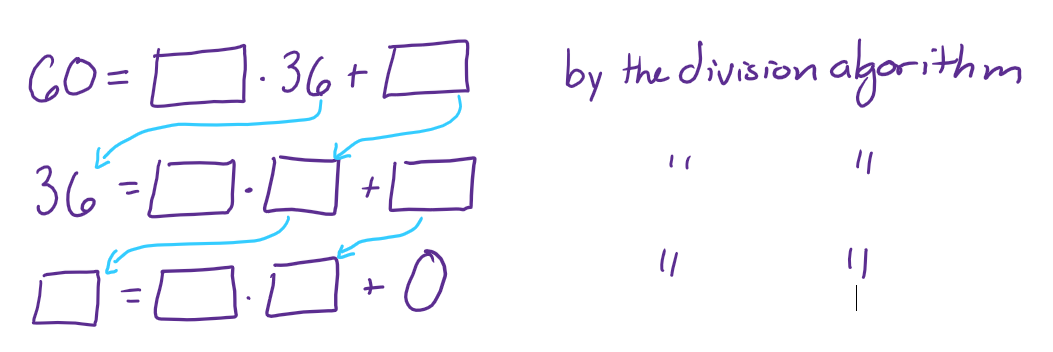
\includegraphics[width=.8\textwidth]{euclid}
			\end{center}
		
		Stop when the remainder is zero.  The previous remainder is the gcd.
	\end{exercise}
}
\slide{
	\begin{exercise}
		Now we know that $\gcd(36,60)=12$ and we want to write 	\[12=36r+60s.\]
		Start with the second to last row of the Euclidean Algorithm:
			\[12=36-1\cdot 24.\]
		Use the line above that to replace 24:
			\[12=36-1\cdot(\underline{\hspace*{1in}}).\]
		Simplify
			\[12=36\cdot(\underline{\hspace*{1in}}) + 60\cdot(\underline{\hspace*{1in}}).\]
	\end{exercise}
}
\slide{
	\begin{defn}
		We say that $m,n\in\Z$ are \emph{relatively prime} if $\gcd(m,n)=1$.
	\end{defn}
	\begin{statementblock}{Theorem 1.2.4}
		Let $m,n\in \Z$ not both zero.  Then
			\begin{center}
				$m,n$ relatively prime $\Leftrightarrow$ $\exists r,s\in\Z$ such that $1=rm+sn$
			\end{center}
	\end{statementblock}
}
\slide{
	\begin{statementblock}{Theorem 1.2.4}
		Let $m,n\in Z$ not both zero.  Then
		\begin{center}
			$m,n$ relatively prime $\Leftrightarrow$ $\exists r,s\in\Z$ such that $1=rm+sn$
		\end{center}
	\end{statementblock}
	\begin{proof}[Proof idea]
		($\Rightarrow$) B\'ezout
		
		($\Leftarrow$) Assume $1=rm+sn$ for some $r,s\in\Z$. Let $c$ be a common divisor of $m$ and $n$.
		\begin{itemize}[label=$\Rightarrow$]
			\item $c\mid(rm+sn)$ \fbox{why}\vskip 2em
			\item $c\mid 1$ \fbox{why}\vskip 2em
			\item $\gcd(m,n)=1$ \fbox{why}
		\end{itemize}
	\end{proof}
}
\slide{\begin{block}{\textbf{Brain Break.}}
	Which superpower would you like to have?
	\vskip .25in
	\begin{minipage}{.5\textwidth}
		\enumarabic{
			\item Mind reading
			\item Invisibility
			\item Teleportation
			\item Flying
			\item \underline{\hspace*{1in}}
			\item I already have a superpower
		}
	\end{minipage}
	%		\begin{minipage}{.4\textwidth}
	%		\mbox{}\hfill\includegraphics[width=2in]{images/mm}
	%		\end{minipage}
\end{block}
}
\slide{
	\begin{statementblock}{Euclid's Lemma}
		Let $p$ be a prime number.
		\enumarabic{
			\item If $p\mid mn$ where $m,n\in\Z$, then $p\mid m$ or $p\mid n$.
			\item If $p\mid m_1m_2\cdots m_r$ where $m_i\in\Z$ for all $i$, then $p\mid m_i\ \exists i$.
		}
	\end{statementblock}
	\begin{nb}
		Proof is in the book. I'll write some examples quick. Think of your own too.
	\end{nb}
}
\slide{
	\begin{statementblock}{Prime Factorization Theorem (Theorem 1.2.7)}
		\enumarabic{
			\item Every integer $n\geq 2$ is a product of (one or more) primes.
			\item This factorization is unique (up to order of the factors).
			
			That is, if
				\[n=p_1p_2\cdots p_r\text{ and }n=q_1q_2\cdots q_2,\]
			then $r=s$ and the $q_j$ can be relabeled so that $p_i=q_i$ for $i=1,2,\dots,r$.
		}
	\end{statementblock}
	\begin{nb}
		I'll walk through the proof of (2) - we'll see similar proofs later in the semester when we talk about UFDs (Unique Factorization Domains).
	\end{nb}
}
\slide{
	\begin{proof}[``Proof'' (1)]
		Strong induction. (See page 26 Example 7.)
	\end{proof}
	\begin{block}{Proof (2)}
		Assume toward contradiction that (2) fails.  Then by \fbox{WOP} there is a smallest integer $m$ such that
			\[m=p_1p_2\cdots p_r=q_1q_2\cdots q_s\]
		are two distinct prime factorizations of $m$.
		
		Thus $m$ is not prime. \fbox{why?}
		So $r,s\geq 2$. 
		
		Notice that
			\[p_1\mid q_1q_2\cdots q_s\text{ so }p_1|q_j\text{ for some }1\leq j\leq s.\]
		\vskip -2em
		\fbox{why?}
	\end{block}
}
\slide{
	\begin{proof}[Proof (2) Continued]
		By relabeling we can assume $p_1\mid q_1$.  Observe that $p_1=q_1$. \fbox{why?}
	
	Since \[m=p_1p_2\cdots p_r=q_1q_2\cdots q_s\text{ and }p_1=q_1,\]
	we see that 
		\[\frac{m}{p_1}=p_2 p_3\cdots p_r=q_2q_3\cdots q_s\]
	are two distinct factorizations of the integer $\frac{m}{p_1}$.
	
	This is a contradiction. \fbox{why?}
	\end{proof}
}
\slide{
	\begin{statementblock}{Corollary}
		Two integers are relatively prime if there exists no prime that divides them both.
	\end{statementblock}
	\begin{statementblock}{Corollary}
		Every $n\in\Z_{\geq 2}$ can be written uniquely as
			\[n=p_1^{n_1}p_2^{n_2}\cdots p_r^{n_r}\]
		where the $p_i$ are distinct primes and $n_i\geq 1$ for all $i$.
	\end{statementblock}
}
\slide{
	\begin{statementblock}{Theorem 1.2.8}
		Let $n\geq 2$ be an integer with prime factorization 
			\[n=p_1^{n_1}p_2^{n_2}\cdots p_r^{n_r},\]
		where the $p_i$ are all distinct primes and $n_i\geq 1$ for all $i$.  Then
			\[d\mid n\Rightarrow d=p_1^{d_1}p_2^{d_2}\cdots p_r^{d_r}\text{ where } 0\leq d_i\leq n_i\ \forall i.\]
	\end{statementblock}
}
\slide{
	\begin{exercise}
		\enumalph{
			\item Write 60 as $p_1^{n_1}p_2^{n_2}\cdots p_r^{n_r}$
			\item Use Theorem 1.2.8 to find all divisors of 60.
		}
	\end{exercise}
	\begin{question}
		How many divisors does $p_1^{n_1}p_2^{n_2}\cdots p_r^{n_r}$ have?
	\end{question}
}
\slide{
	\begin{statementblock}{Theorem 1.2.9}
		Let $\{a,b,c,\dots\}$ be a finite set of positive integers and write
			\begin{eqnarray*}
				a&=&p_1^{a_1}p_2^{a_2}\cdots p_r^{a_r}\\
				b&=&p_1^{b_1}p_2^{b_2}\cdots p_r^{b_r}\\
				c&=&p_1^{c_1}p_2^{c_2}\cdots p_r^{c_r}
			\end{eqnarray*}
		where there is an exponent of zero if the prime is not a factor.
		
		Then 
			\[\gcd(a,b,c,\dots)=p_1^{k_1}p_2^{k_2}\cdots p_r^{k_r},\]
		where $k_i=\min(a_i,b_i,c_i,\dots)$ for each $i$, and
			\[\operatorname{lcm}(a,b,c,\dots)=p_1^{m_1}p_2^{m_2}\cdots p_r^{m_r},\]
		where $m_i=\max(a_i,b_i,c_i,\dots)$ for each $i$.
	\end{statementblock}
}
\slide{
	\begin{exercise}
		\[28665=3^2\cdot5\cdot7\cdot13\text{ and }22869=3^3\cdot7\cdot 11^2\]
		Compute
			\enumalph{
				\item $\gcd(28665,22869)$
				\item $\operatorname{lcm}(28665,22869)$
			}
	\end{exercise}
}
\end{document}

